The following section describes the workings of the tool. If you
intend to use the tool a lot or extend it, it is important that you
read this section.  Some Definitions before we start:
\begin{itemize}
\item Workflow: A sequence of steps involved in moving from a
  beginning state to an ending state.
\item Scientific Workflow Application: An application that automates a
  workflow process through software, with each step in the workflow
  being performed by a separate “scientific” software application.
\item Scientific Workflow System software providing an infrastructure
  for the set-up, scheduling, running, and monitoring of a user
  defined scientific workflow application.
\end{itemize}

The \texttt{EE-UQ} application is a very limited scientific workflow system
that allows users to create scientific workflow applications needed
for the characterization of the response of a building subjected to
earthquake ground motions. It allows the users to then create and run
the workflow application using the data of the users choosing. The
application itself is composed of two parts:

\begin{itemize}
\item Frontend User Interface (UI): This is the application the user
  interacts with to create a building description and
  specify which workflow to run, i.e. given the building, the user
  chooses which applications to use and what data to use for the
  different applications; see \Cref{chap:usage}. As shown in \Cref{fig:figure17}, it 
  creates an input file for the workflow, the BIM, and starts the workflow running.  
\item Backend Application: This is the application that actually
  creates and runs the workflow. It consists of a script that
  processes the output file from the UI to determine the applications
  to run and their data, it invokes these applications using the
  outputs from one application as the input to another. The
  application that is run is a python script, \texttt{EE-UQ.py}, that can be
  found in the /applications/Workflow/ directory.  The input and
  output from each application is in the form of JavaScript Object
  Notation (\texttt{JSON}) files. \texttt{JSON} is a human readable file format used
  widely for passing data between your front-end browser application
  (Safari, Firefox, Internet Explorer) and backend servers.
\end{itemize}


\begin{figure}[!htbp]
  \centering {
    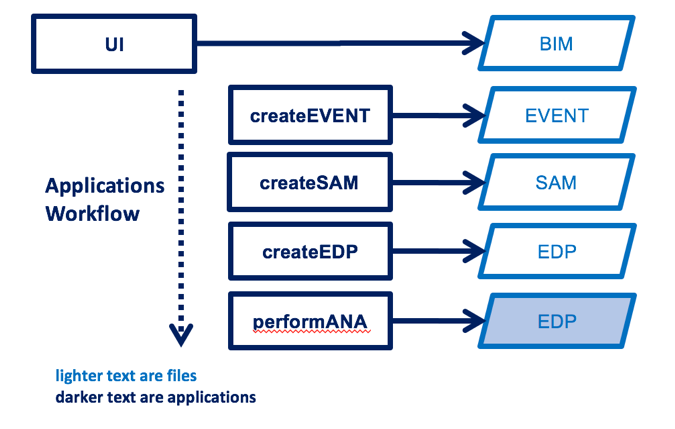
\includegraphics[width=0.8\textwidth]
    {theory_and_implementation/figures/workflowWithoutUQ.png} }
  \caption{Workflow without uncertainty quantification}
  \label{fig:figure17}
\end{figure}


In the absence of uncertainty, the applications that are invoked by
this script are categorized into certain types of applications, as shown 
in \Cref{fig:figure17}:
\begin{enumerate}
\item createEVENT: given the structure and the user input for hazard
  application, define the loadings for the building, i.e. the ground
  motions for an earthquake event. The output file is an EVENT file.
\item createSAM: given the building description and event, create a
  finite element model of the building. The output file is a SAM
  (Structural Analysis Model) file.
\item createEDP: given the building, determine what output quantities
  are required. The output file is the EDP (engineering Demand
  Parameters) file.
\item performANA: given the finite element model and the event,
  perform a finite element simulation. The responsibility of the
  performANA is to fill in the values in the EDP files.
\end{enumerate}


The need to characterize the uncertainties in the computed response
complicates this workflow. This is because the uncertainties in the
inputs, random variables and random field variables, may exist for
each application, e.g. Young’s modulus in the building input file,
magnitude of event or event ground motion in createEVENT, finite
element material properties in createSAM, and integration scheme,
damping ratio or convergence tolerance in performANA.

\begin{figure}[!htbp]
  \centering {
    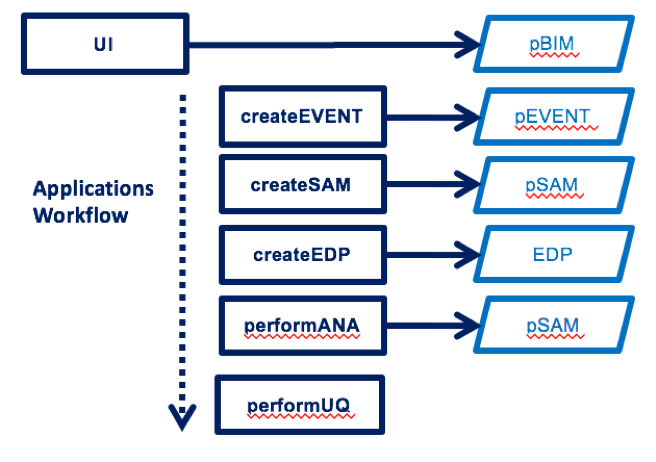
\includegraphics[width=0.8\textwidth]
    {theory_and_implementation/figures/workflowWithUQ.png} }
  \caption{Workflow with uncertainty quantification}
  \label{fig:figure18}
\end{figure}

As a consequence, each application is called with two different sets of
input arguments. The first time the application is invoked with a
“–getRV” input argument. This tells the application to return
information about the random variables inside a “randomVariables”
entry in the p output file generated by the application along with
other needed data, e.g. the event type. The randomVariables is a
\texttt{JSON array} of random variables, each with a field for a name,
a type, a value, and other info that depends on the type, e.g. \\ \\


\begin{lstlisting}
{
  "randomVariables": [
        {
            "distribution": "Normal",
            "mean": 6,
            "name": "fc",
            "stdDev": 0.6,
            "value": "RV.fc",
            "variableClass": "Uncertain"
        },
        {
            "distribution": "Normal",
            "mean": 60,
            "name": "fy",
            "stdDev": 6,
            "value": "RV.fy",
            "variableClass": "Uncertain"
        },
        {
            "distribution": "Normal",
            "mean": 30000,
            "name": "E",
            "stdDev": 3000,
            "value": "RV.E",
            "variableClass": "Uncertain"
        }

}
\end{lstlisting}

It is during the running of the UQ engine that the value field in
these random variables are filled in. Initially as shown, the value
field contains RV.variableName.  This is required must because it is used by
the UQ engine to set the value. When the application is called
again by the UQ engine during it’s running, the application is
called without the “-getRV”. The application finds these value fields
now set to numbers (or strings) in the pFiles. \\

The performUQ application is actually a script that calls 3
applications, as shown below and illustrated in \Cref{fig:uq_sampling}:
\begin{enumerate}
\item PreProcessUQ: to  parse all the pFiles to build the
  list of all random variables.
\item PeformUQ: to invoke the UQ engine, which for the number of
  samples specified will fill in the random variable values, run the
  applications in the workflow with the new files.
\item PostProcessUQ: to process all the output results, filling in
  the EDP’s
\end{enumerate}

\begin{figure}[!htbp]
  \centering {
    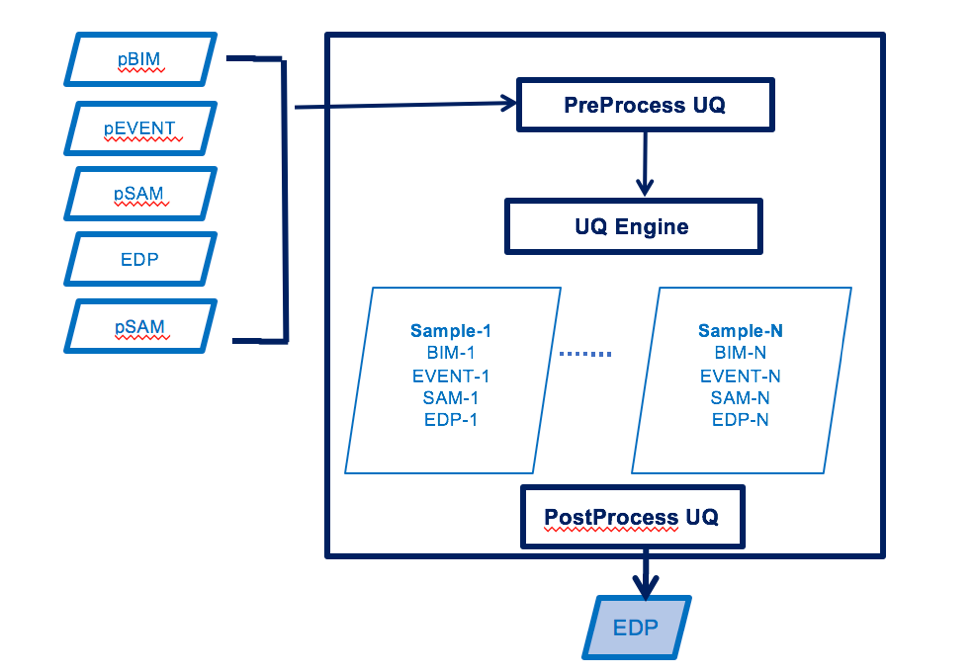
\includegraphics[width=0.8\textwidth]
    {theory_and_implementation/figures/uq_sampling.png} }
  \caption{UQ sampling}
  \label{fig:uq_sampling}
\end{figure}

PerformUQ is the computationally expensive part of the simulation. 
As discussed earlier, the user has the option of running
locally or remotely at DesignSafe. When the user selects to run the
job remotely, it is the PerformUQ operation that is run
remotely. The operations peformed in the PreProcessUQ and PostProcessUQ stages are run locally.
